\documentclass[10pt]{beamer}
\usepackage[slovene]{babel}
\usepackage[utf8]{inputenc}
\usepackage[T1]{fontenc}
\usepackage{lmodern}
\usepackage{mathptmx}
\usepackage{helvet}
\usepackage{courier}
\usepackage{hyperref}
\usepackage{tikz}
\usepackage{enumerate}
\setbeamertemplate{caption}[numbered]

\usetheme{CambridgeUS}

\setbeamercolor*{item}{fg=red}
\setbeamercolor*{label}{fg=red}

\begin{document}


\title[Reševanje problema trgovskega potnika s k-optimalnim in
Lin-Kernighanovim algoritmom]{Reševanje problema trgovskega potnika s k-optimalnim in
Lin-Kernighanovim algoritmom}
\author[Žan Jernejčič in Ines Šilc]{Žan Jernejčič in Ines Šilc}
\institute [FMF]{Fakulteta za matematiko in fiziko}

\begin{frame}
	\titlepage
\end {frame}

\begin{frame}

\begin{columns}
\column{0.5\textwidth}

\begin{minipage}[c][0.4\textheight][c]{\linewidth}
  \begin{figure}
  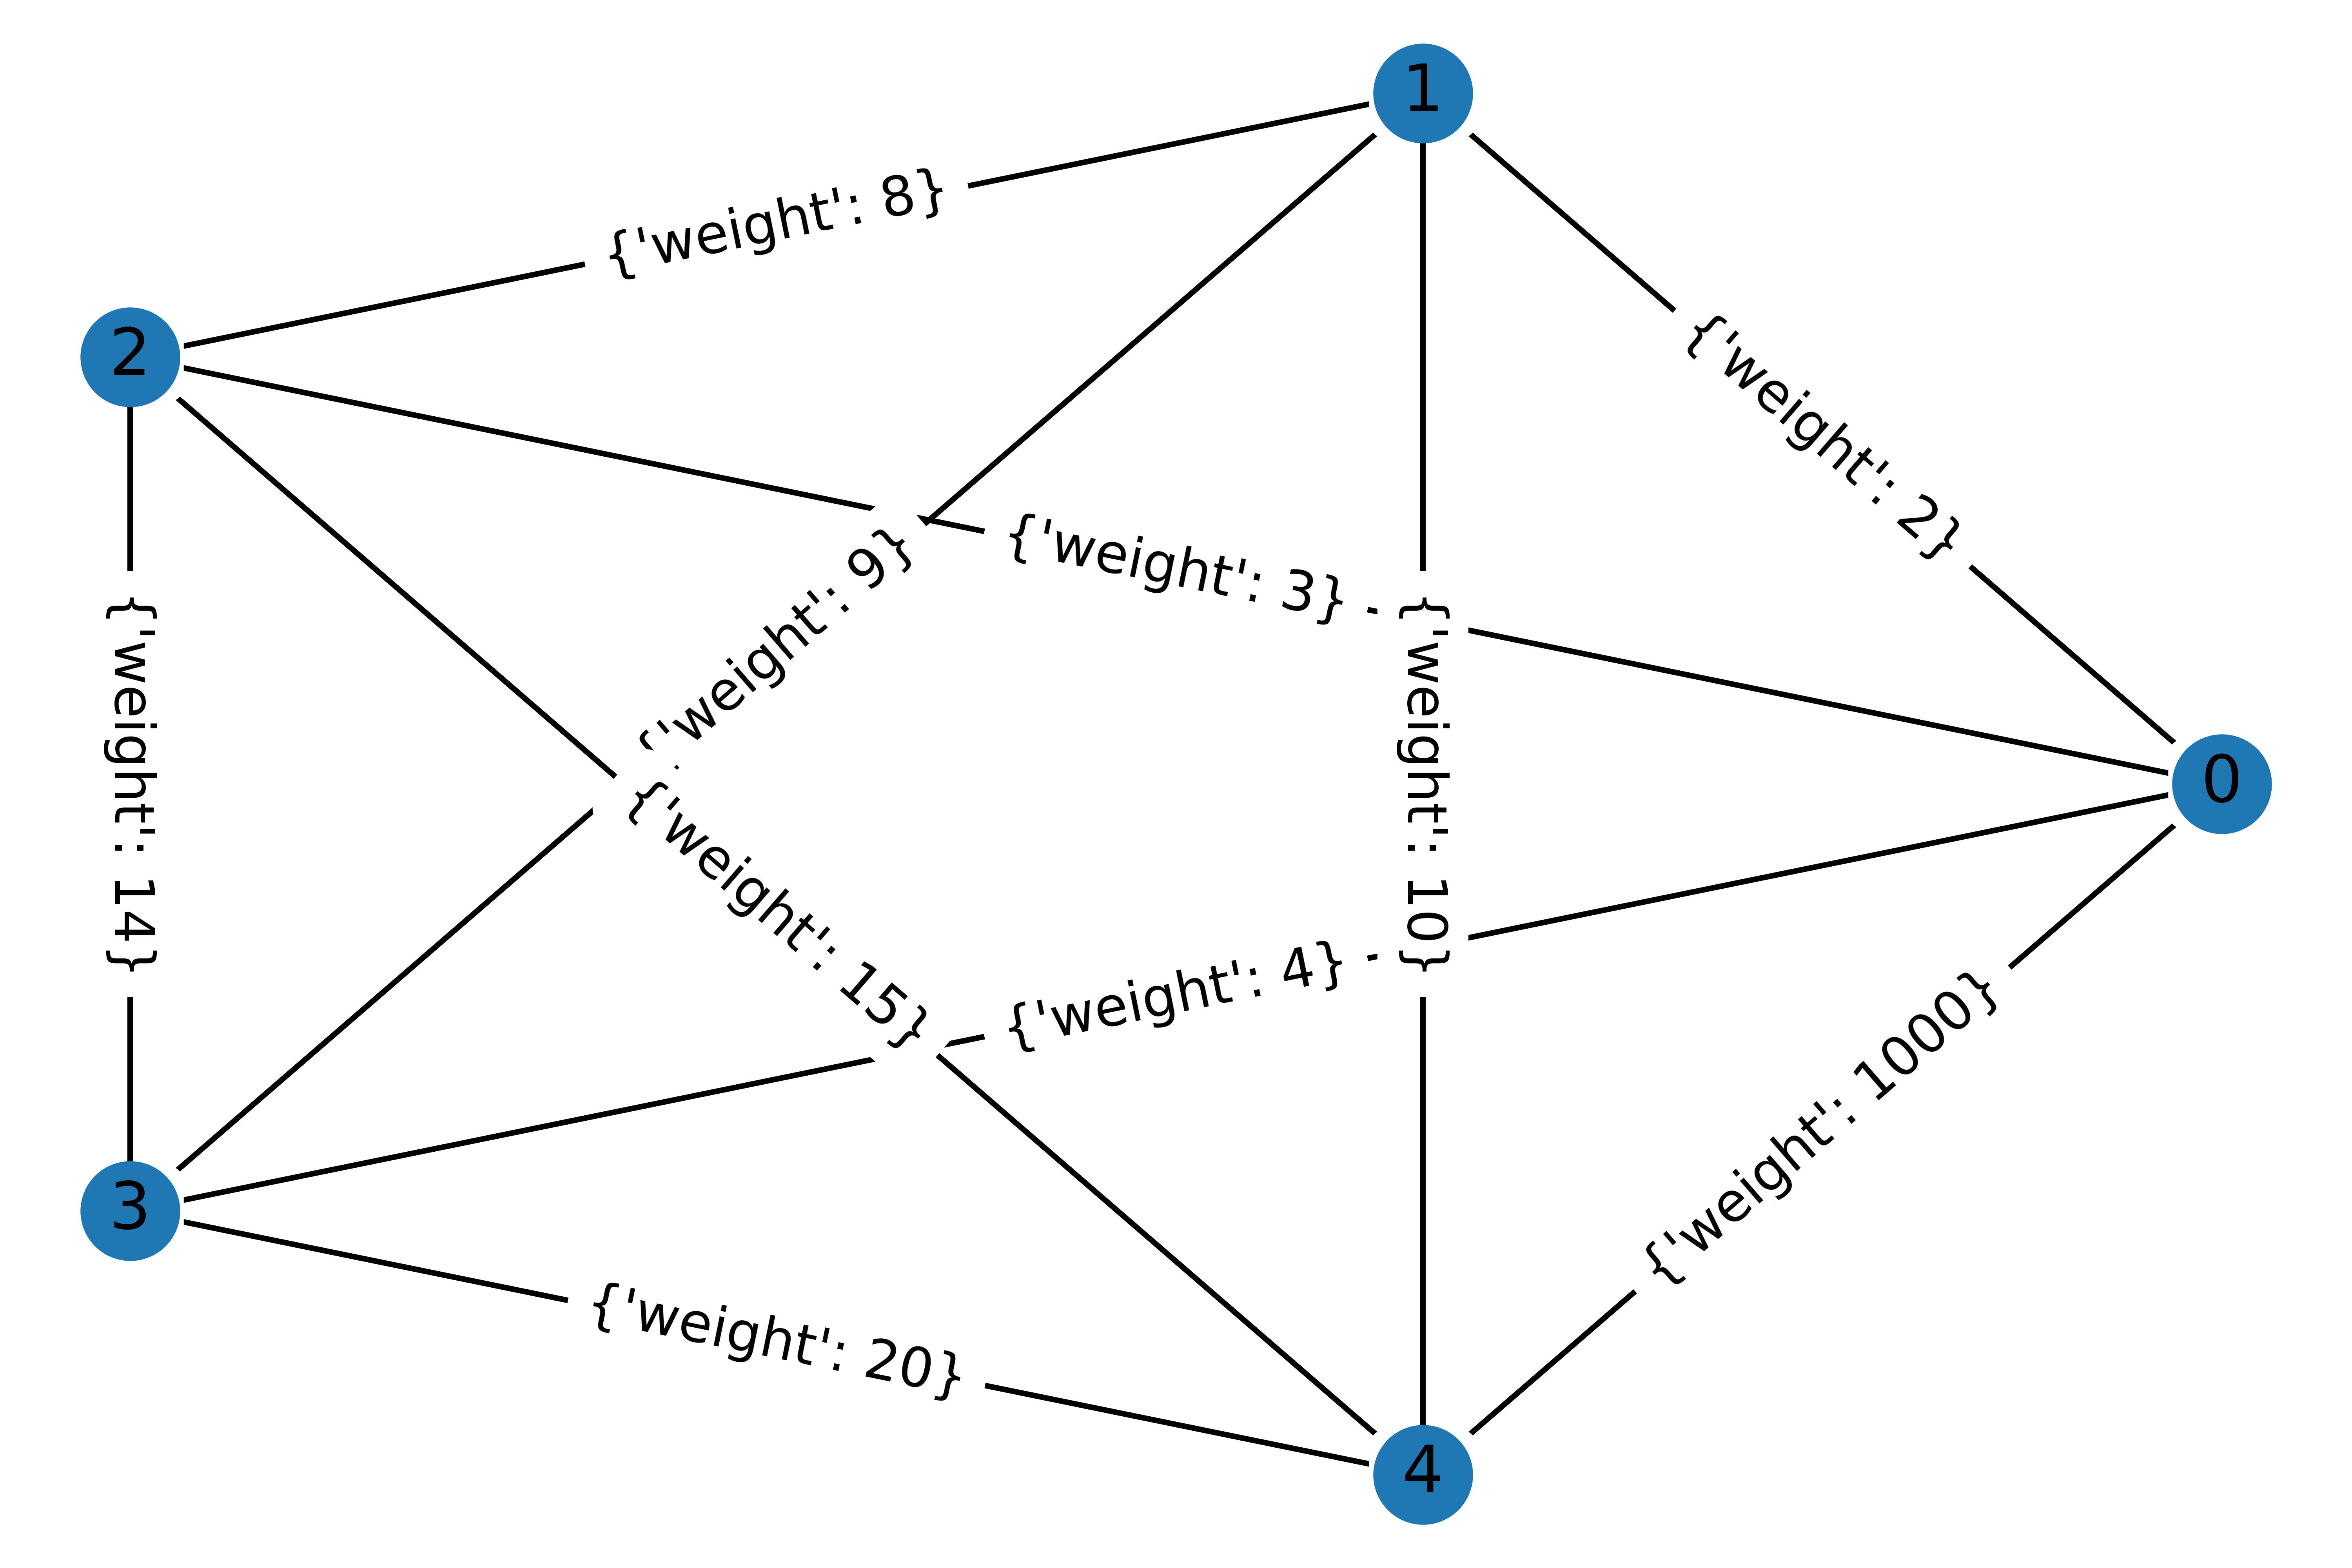
\includegraphics[width=0.8\linewidth]{primeri/primer1.png}
 	\caption{Poln graf na 5 vozliščih}
	\label{Slika 1}
	\end{figure}
\end{minipage}

\begin{minipage}[c][0.4\textheight][c]{\linewidth}
  \begin{figure}
  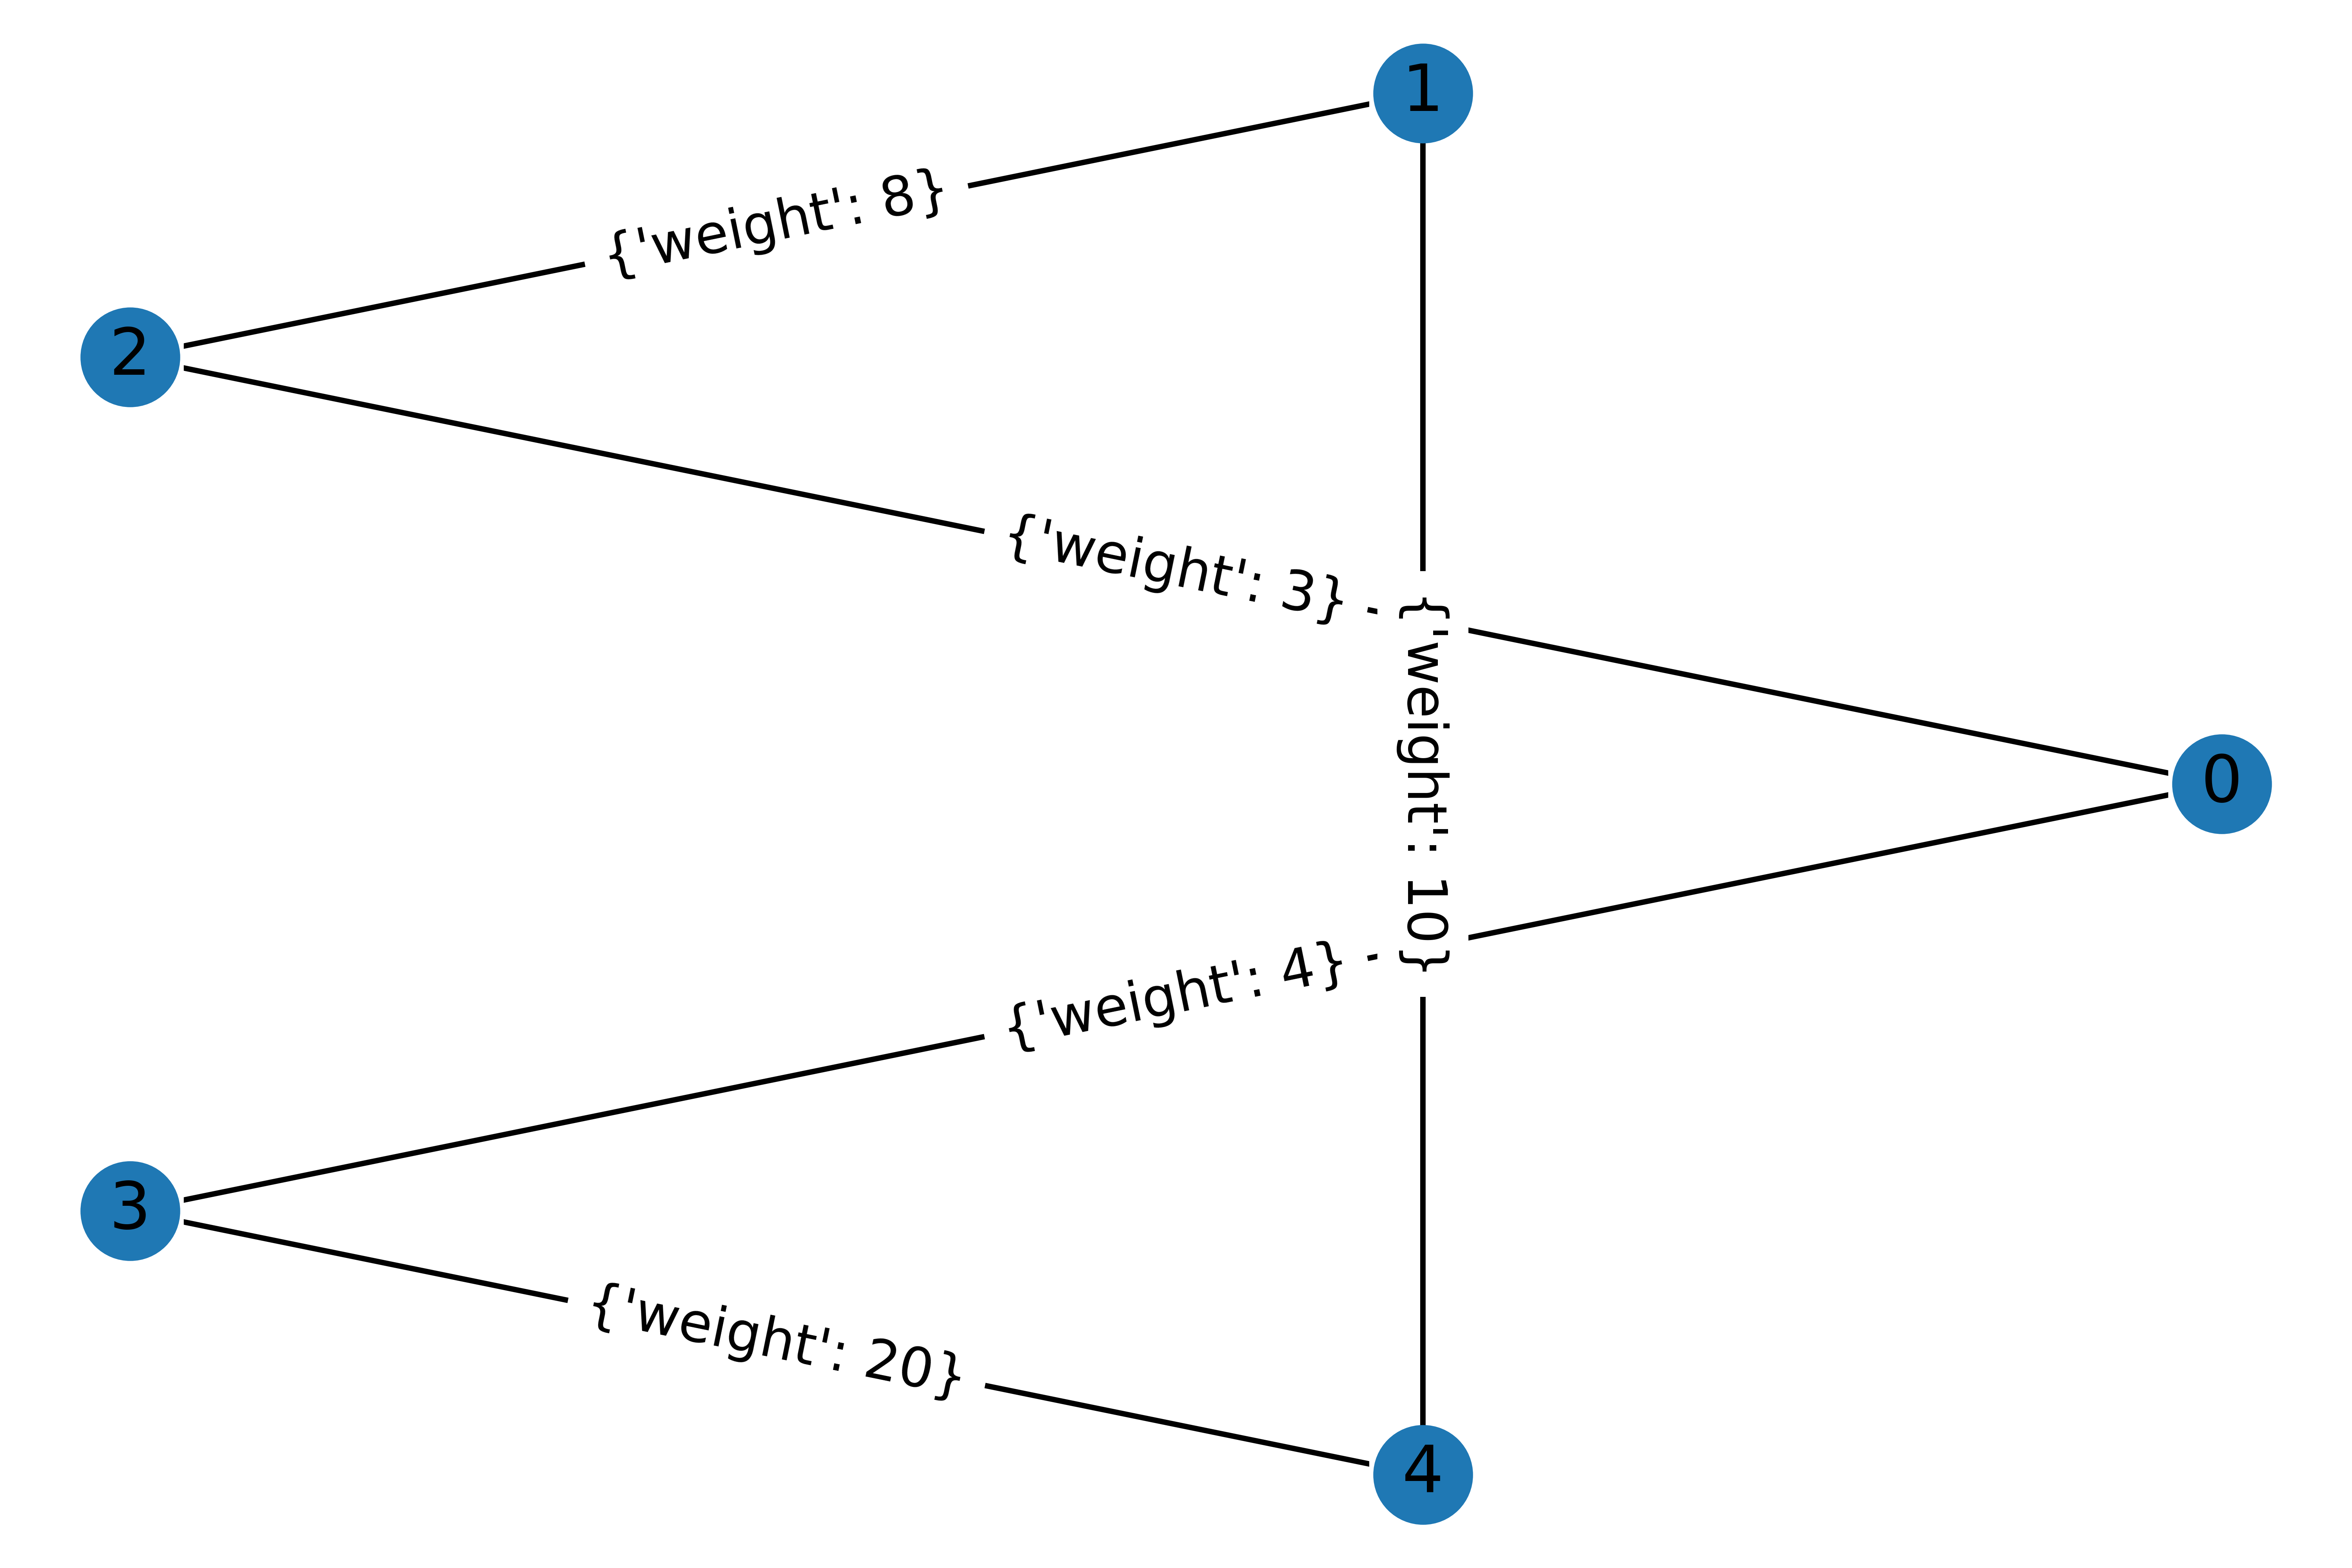
\includegraphics[width=0.8\linewidth]{primeri/primer1_3opt.png}
 	\caption{3-opt}
	\label{Slika 3}
	\end{figure}
\end{minipage}

\column{0.5\textwidth}
\begin{minipage}[c][0.4\textheight][c]{\linewidth}
\begin{figure}
  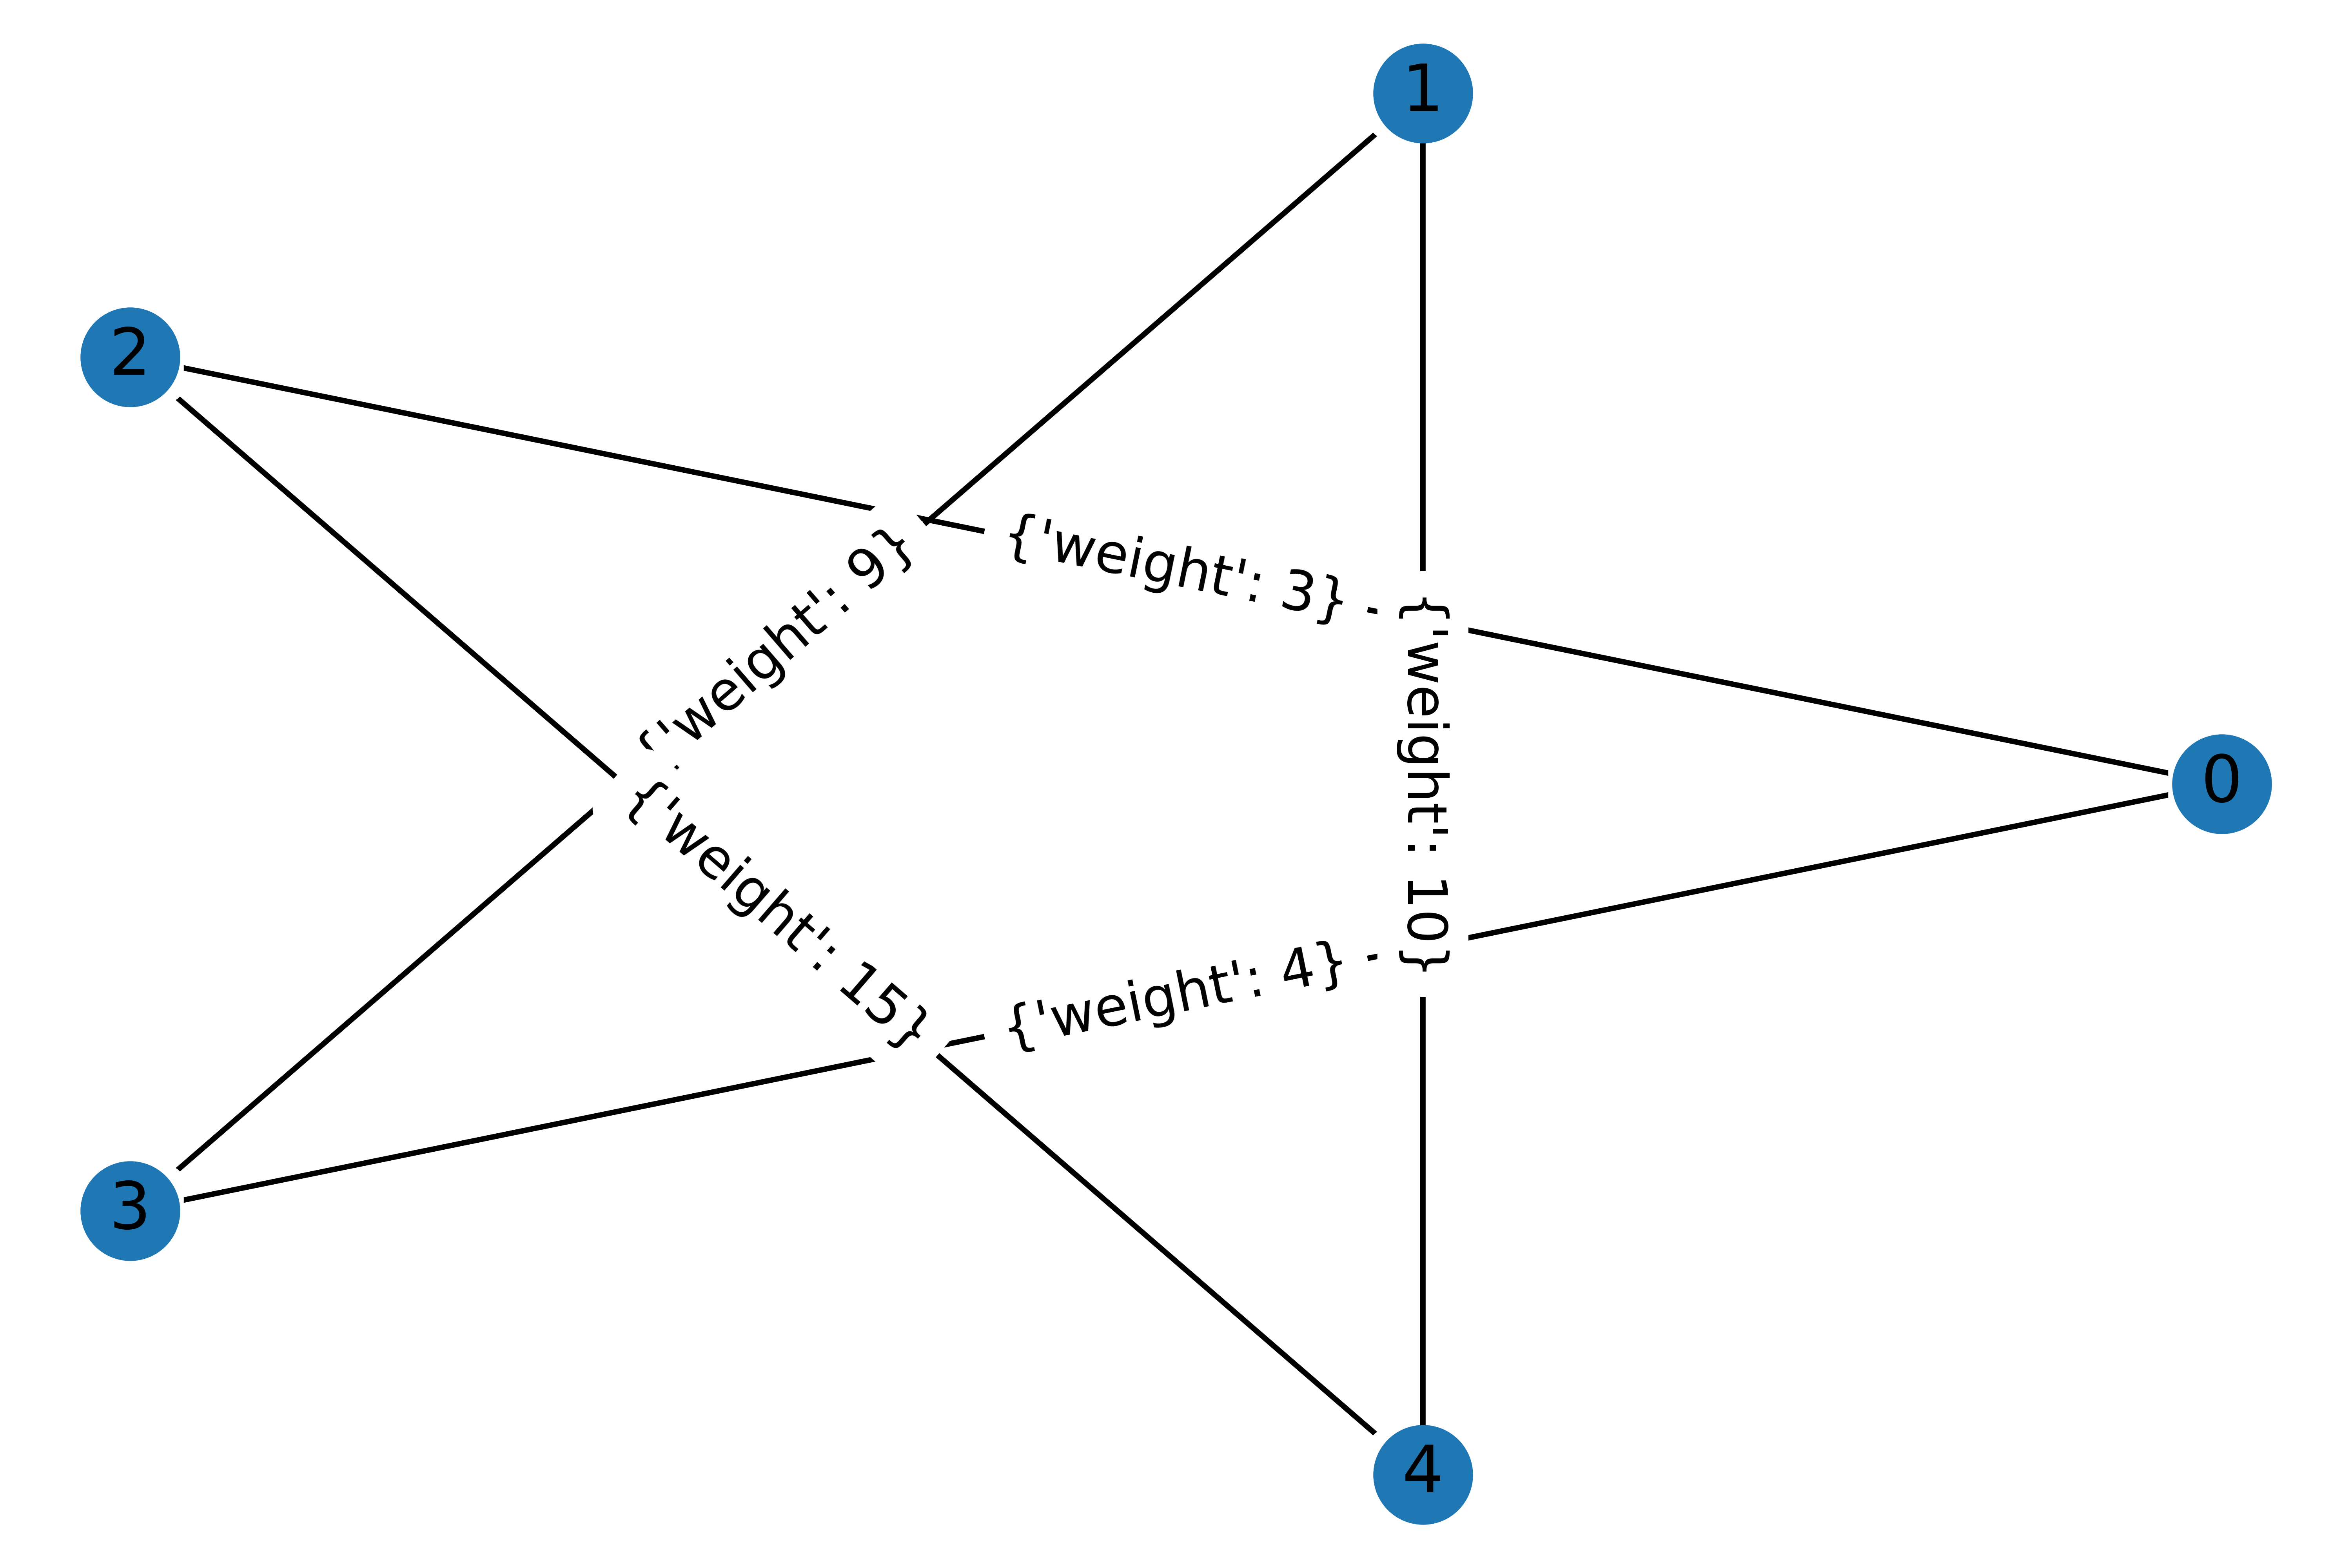
\includegraphics[width=0.8\linewidth]{primeri/primer1_2opt.png}
\caption{2-opt}
\label{Slika 2}
\end{figure}
\end{minipage}

\begin{minipage}[c][0.4\textheight][c]{\linewidth}
\begin{figure}
  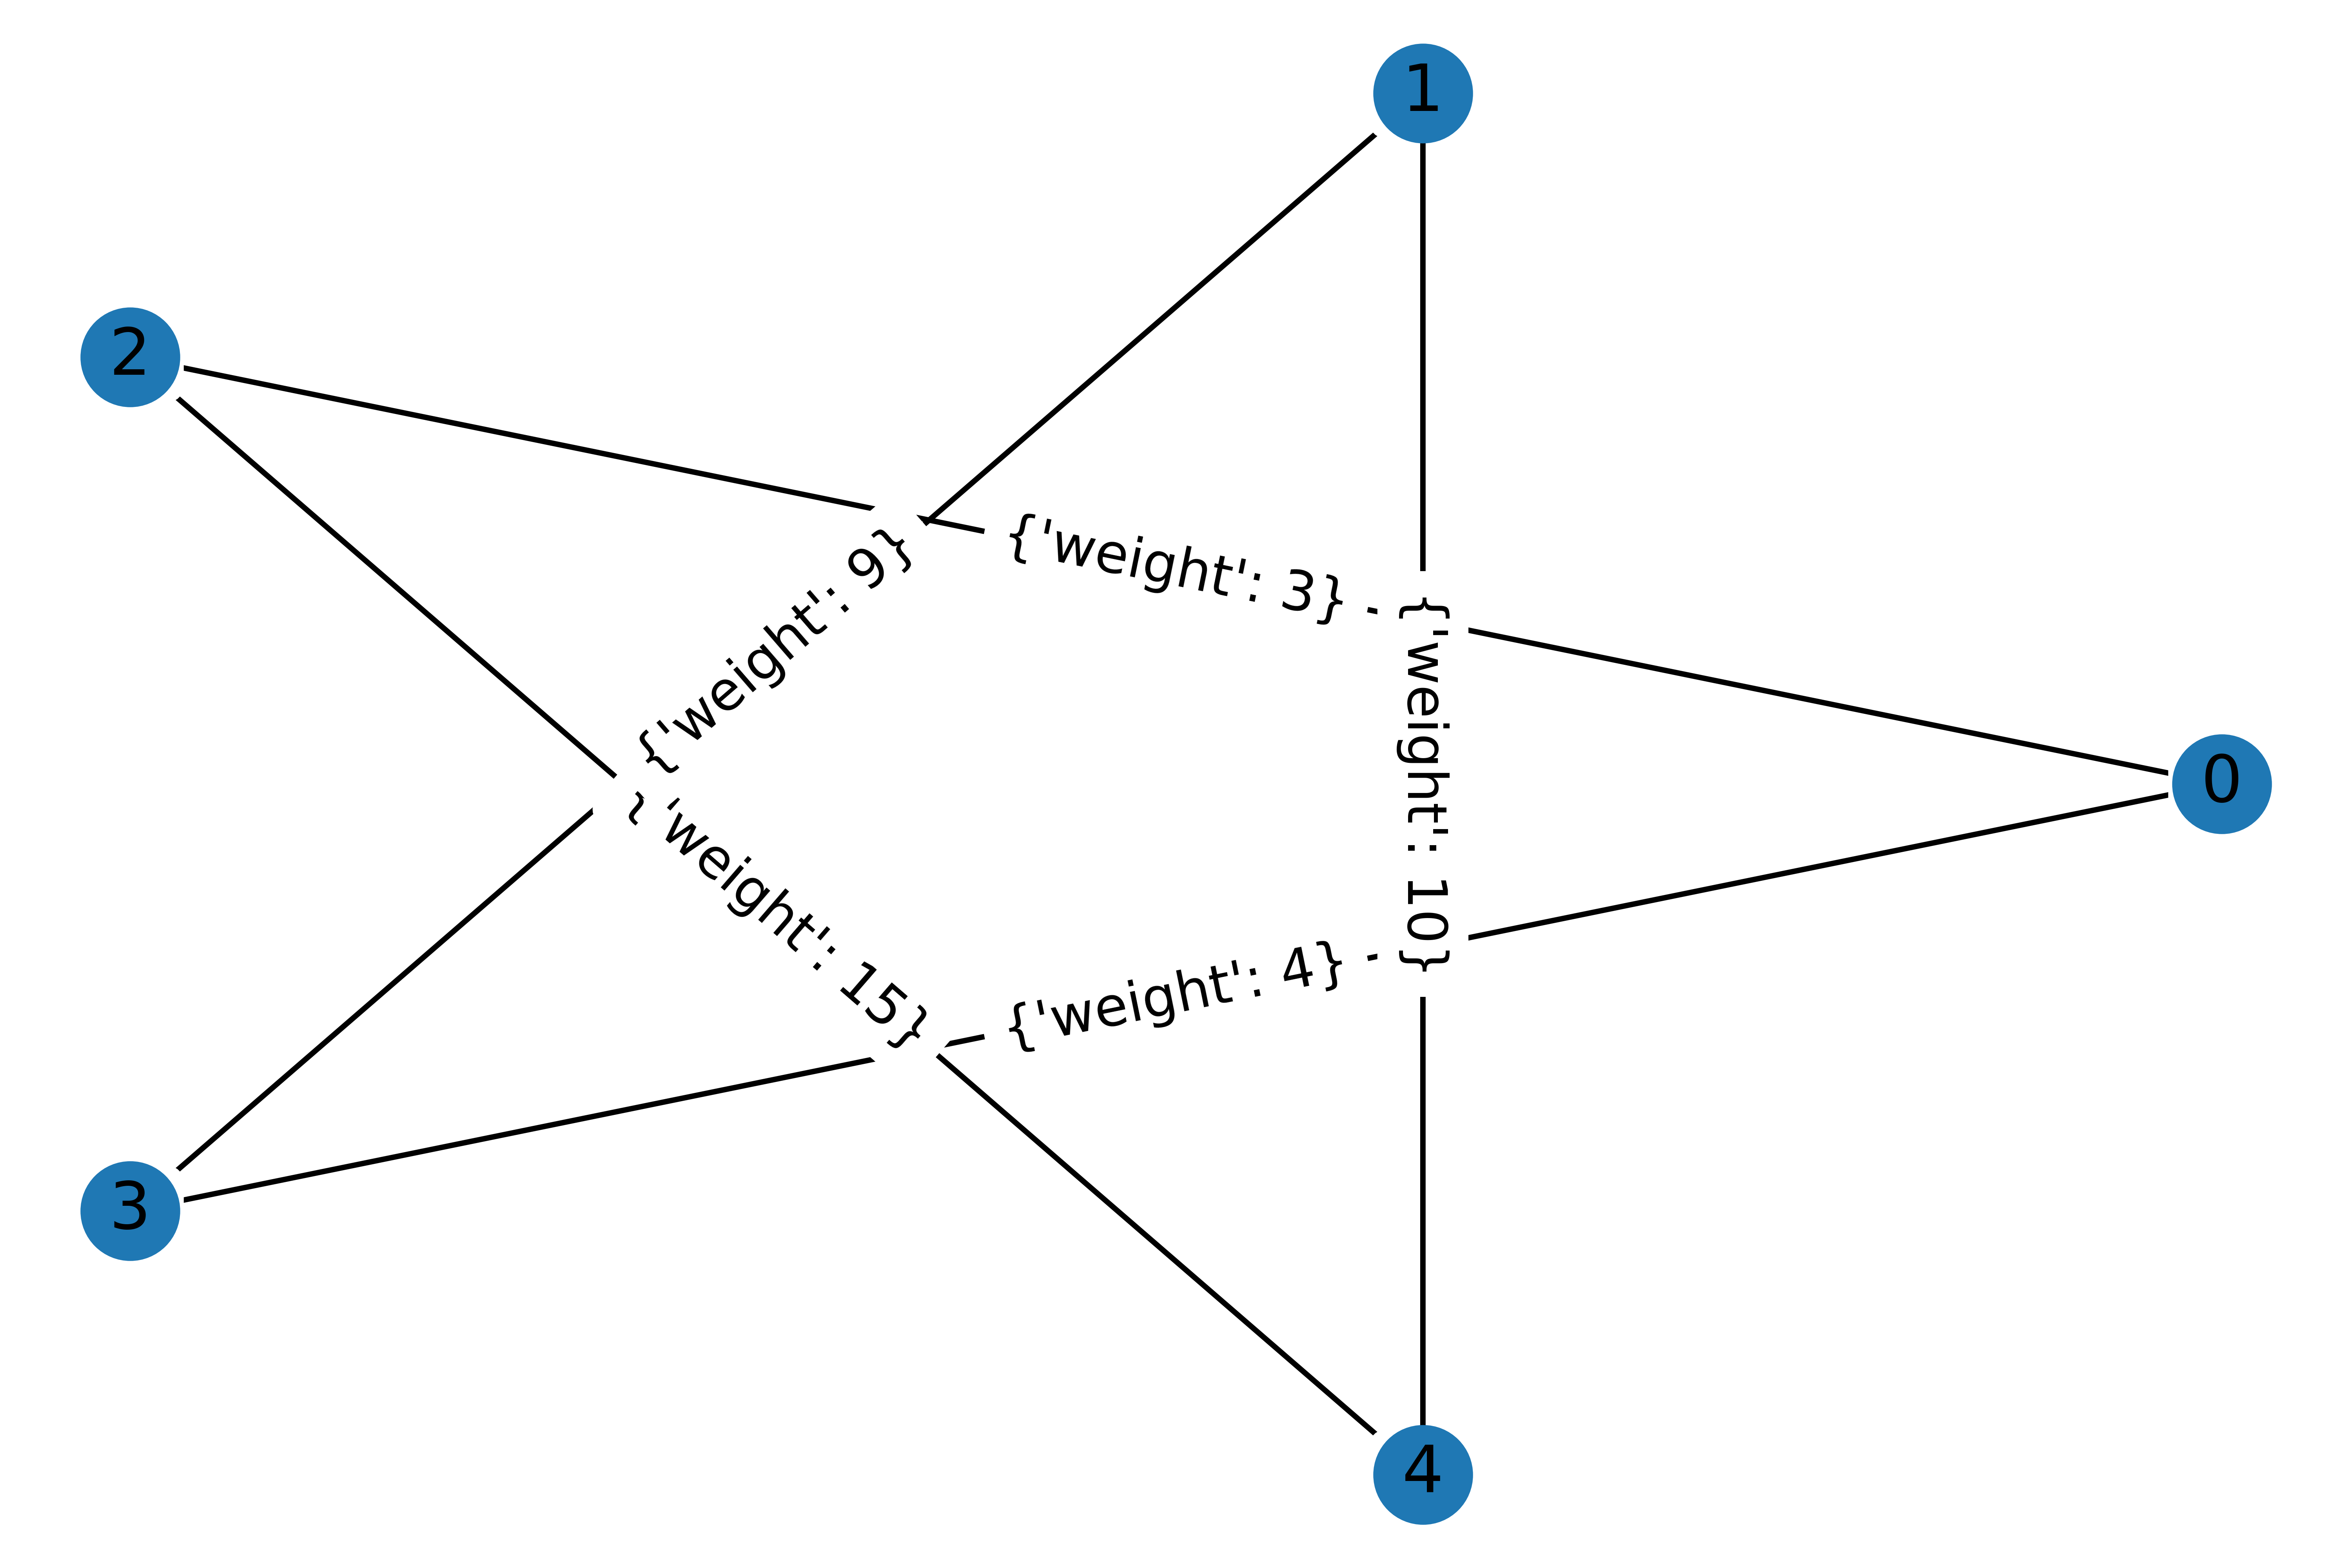
\includegraphics[width=0.8\linewidth]{primeri/primer1_lk.png}
\caption{LK}
\label{Slika 4}
\end{figure}
\end{minipage}
\end{columns}

\end{frame}

\begin{frame}

\begin{columns}
\column{0.5\textwidth}

\begin{minipage}[c][0.4\textheight][c]{\linewidth}
  \begin{figure}
  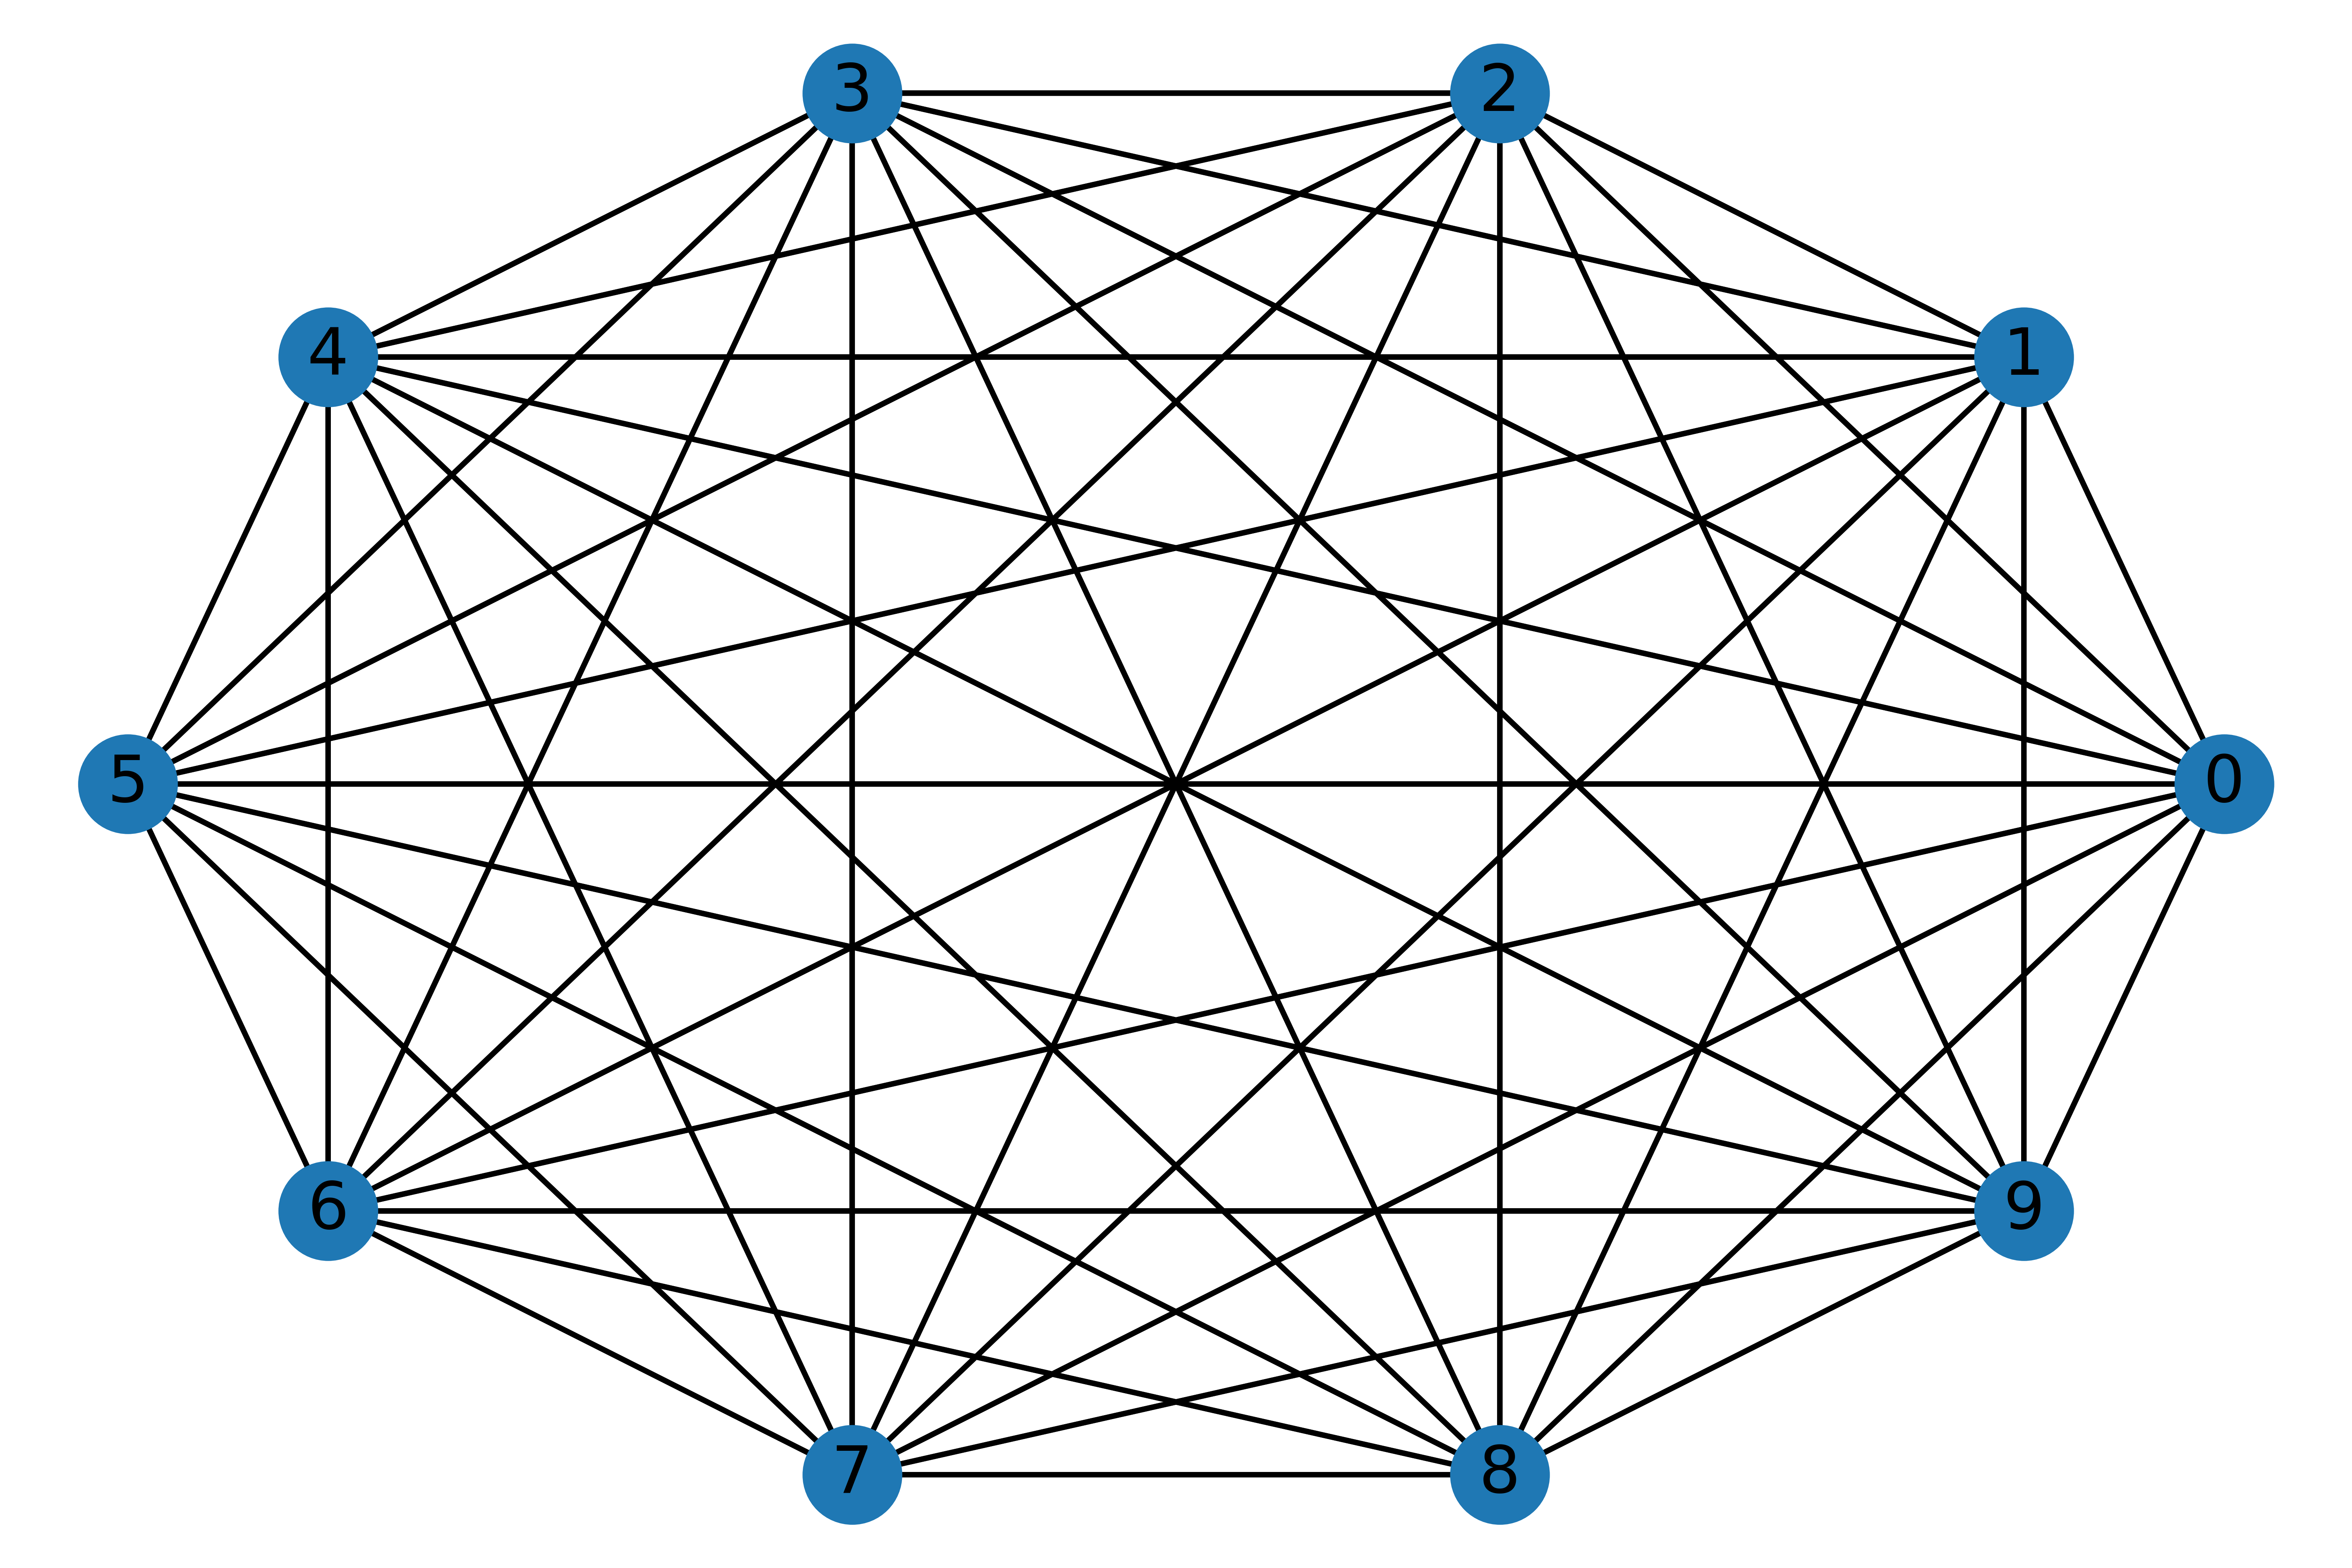
\includegraphics[width=0.8\linewidth]{primeri/primer2.png}
 	\caption{Poln graf na 5 vozliščih}
	\label{Slika 5}
	\end{figure}
\end{minipage}

\begin{minipage}[c][0.4\textheight][c]{\linewidth}
  \begin{figure}
  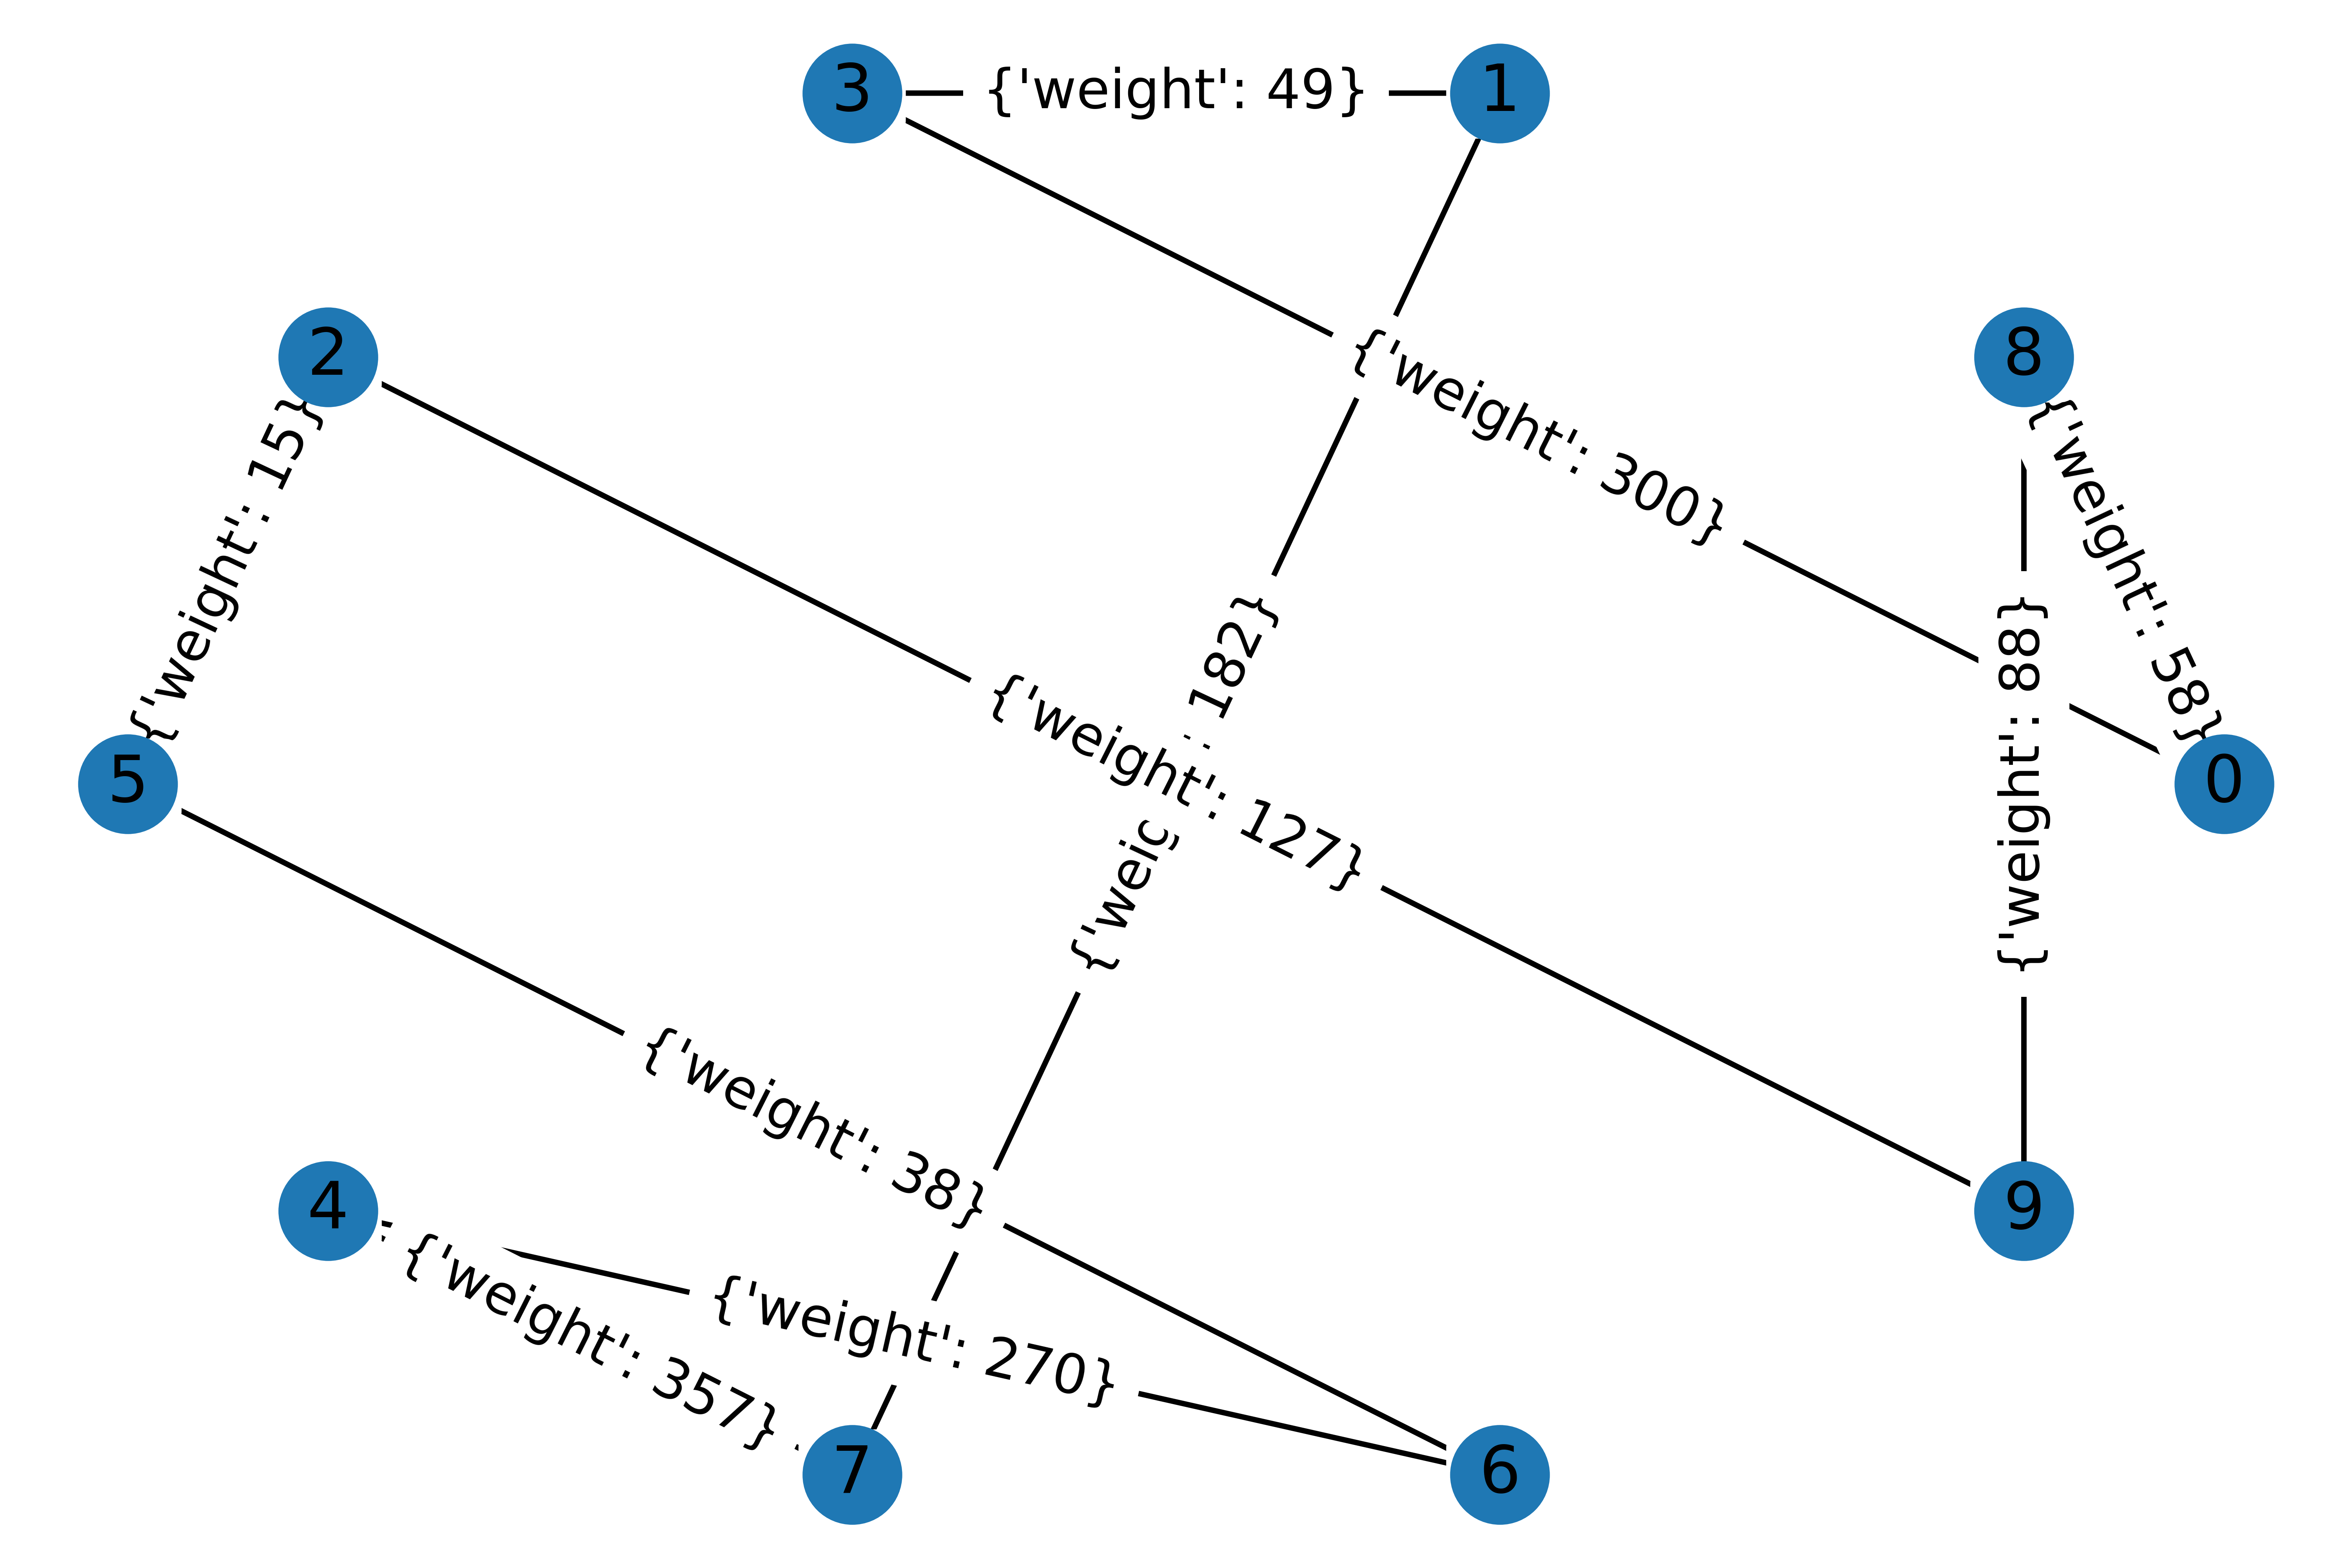
\includegraphics[width=0.8\linewidth]{primeri/primer2_3opt.png}
 	\caption{3-opt}
	\label{Slika 7}
	\end{figure}
\end{minipage}

\column{0.5\textwidth}
\begin{minipage}[c][0.4\textheight][c]{\linewidth}
\begin{figure}
  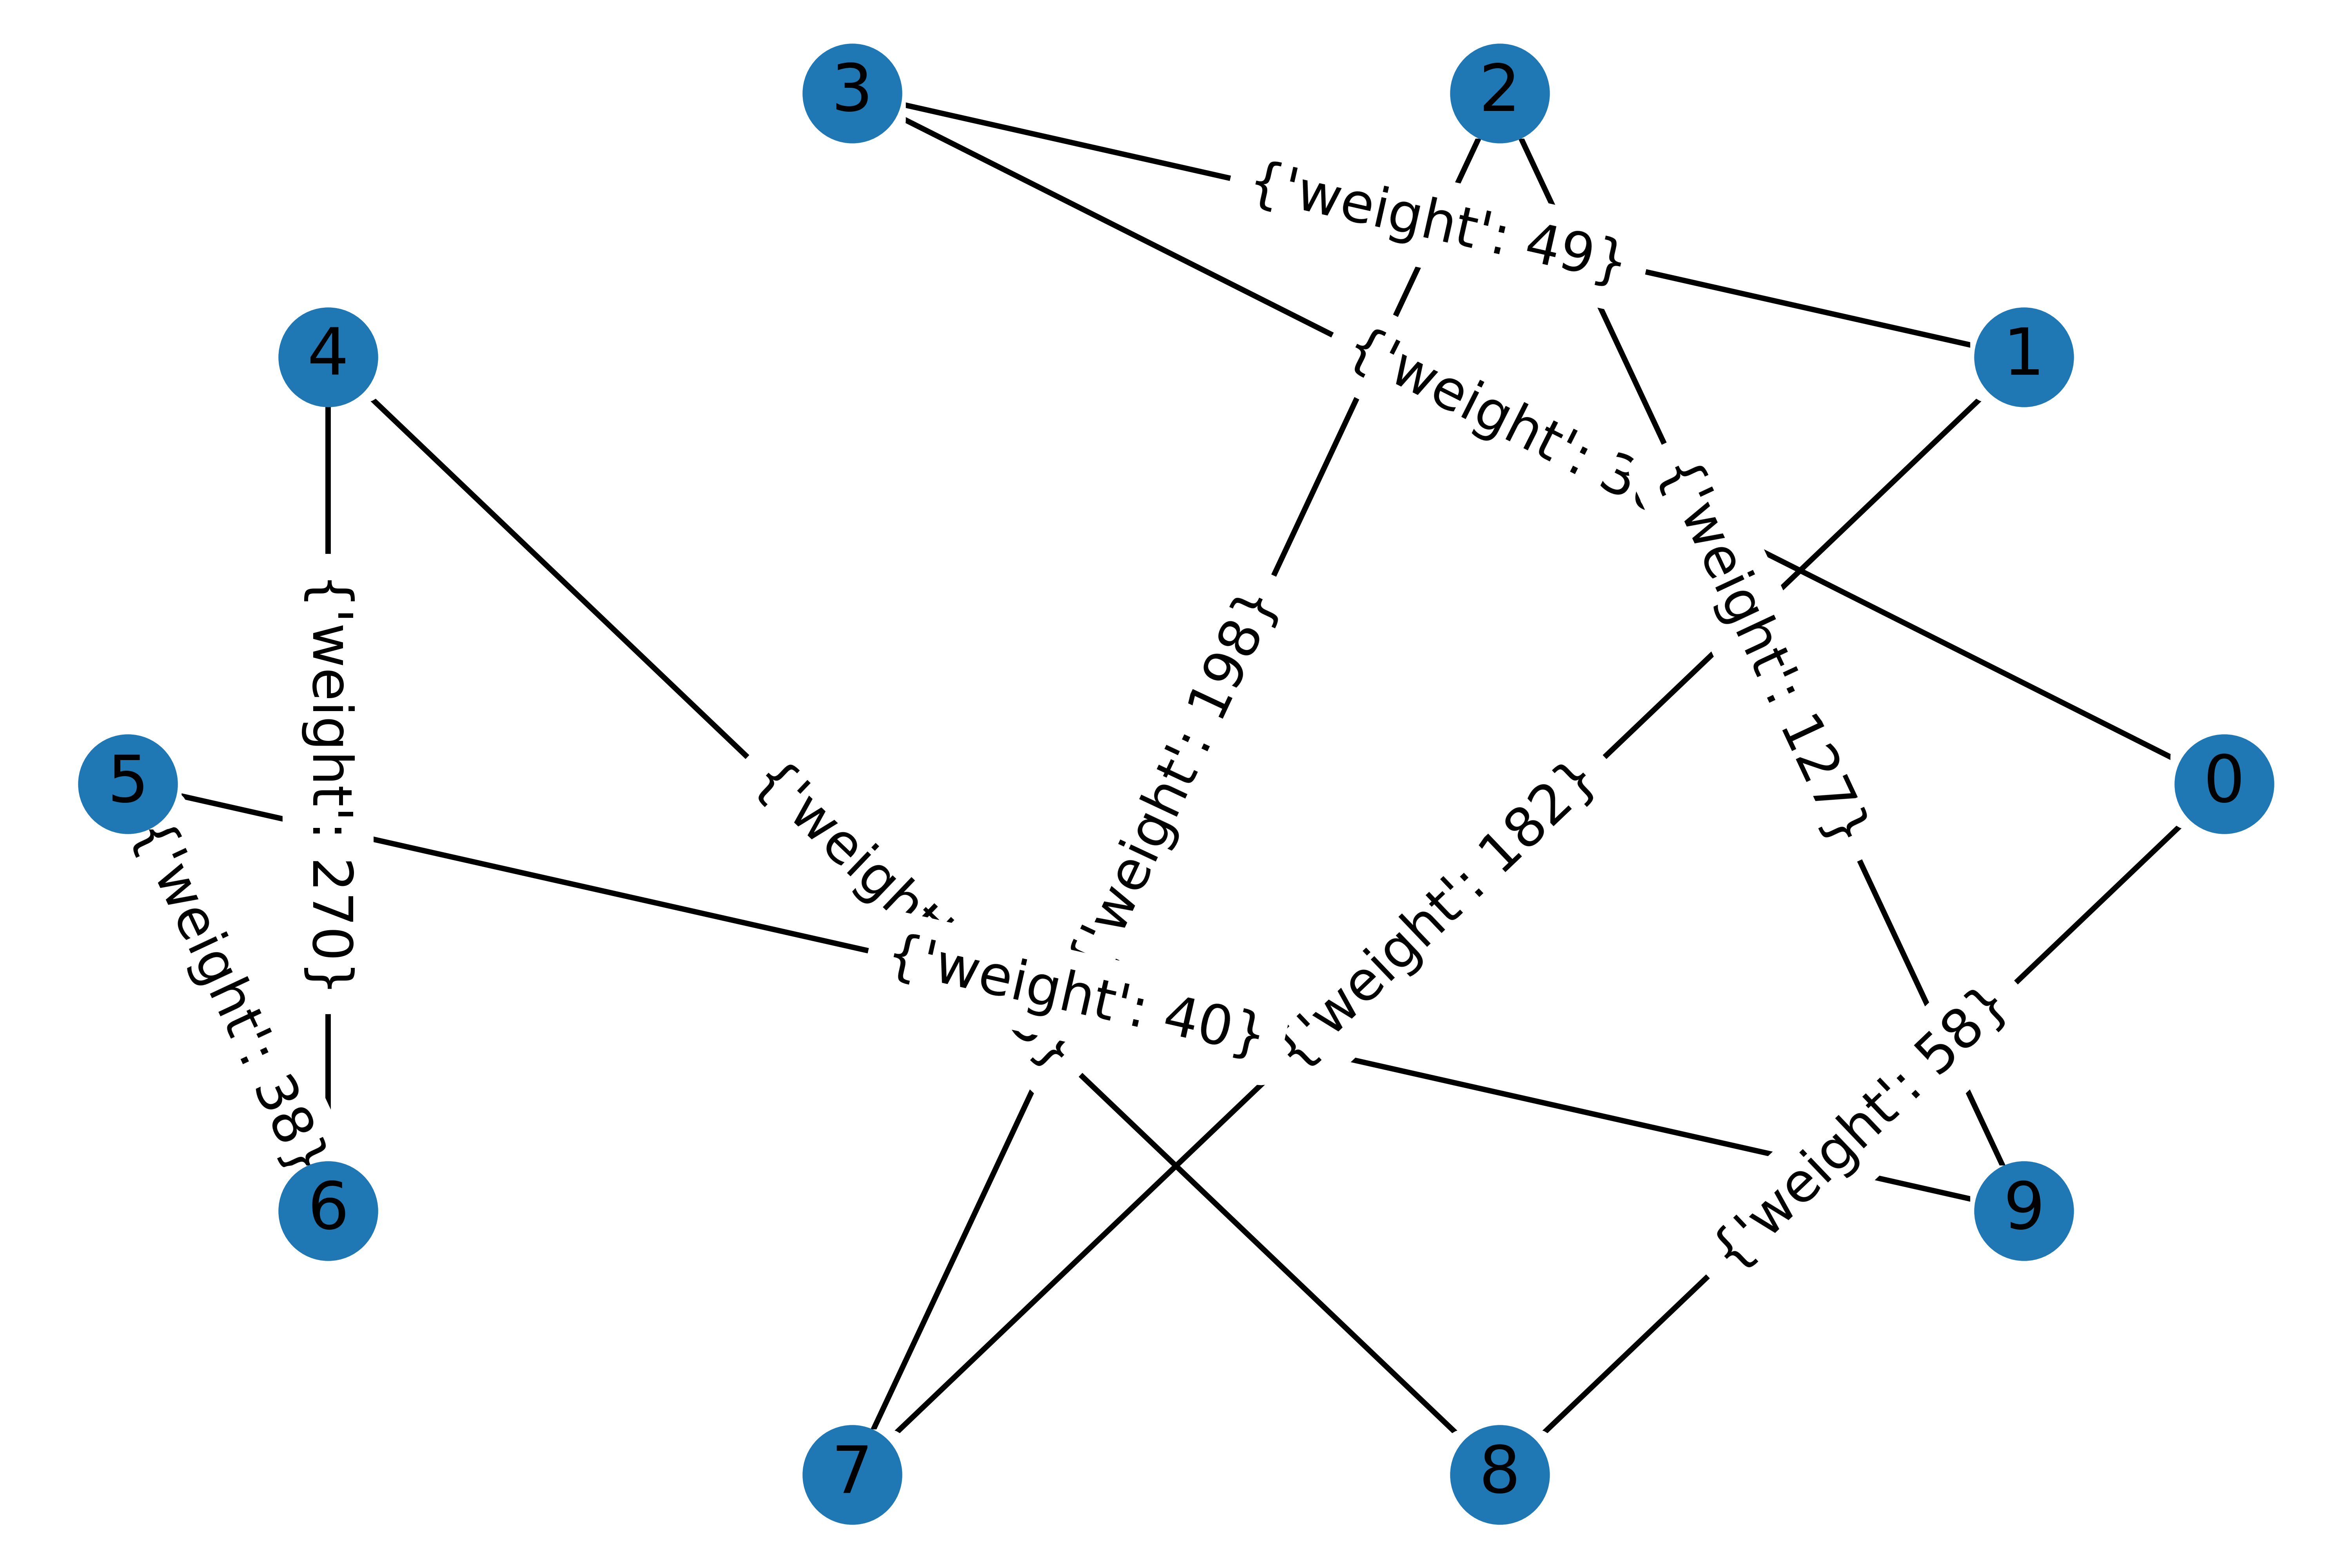
\includegraphics[width=0.8\linewidth]{primeri/primer2_2opt.png}
\caption{2-opt}
\label{Slika 6}
\end{figure}
\end{minipage}

\begin{minipage}[c][0.4\textheight][c]{\linewidth}
\begin{figure}
  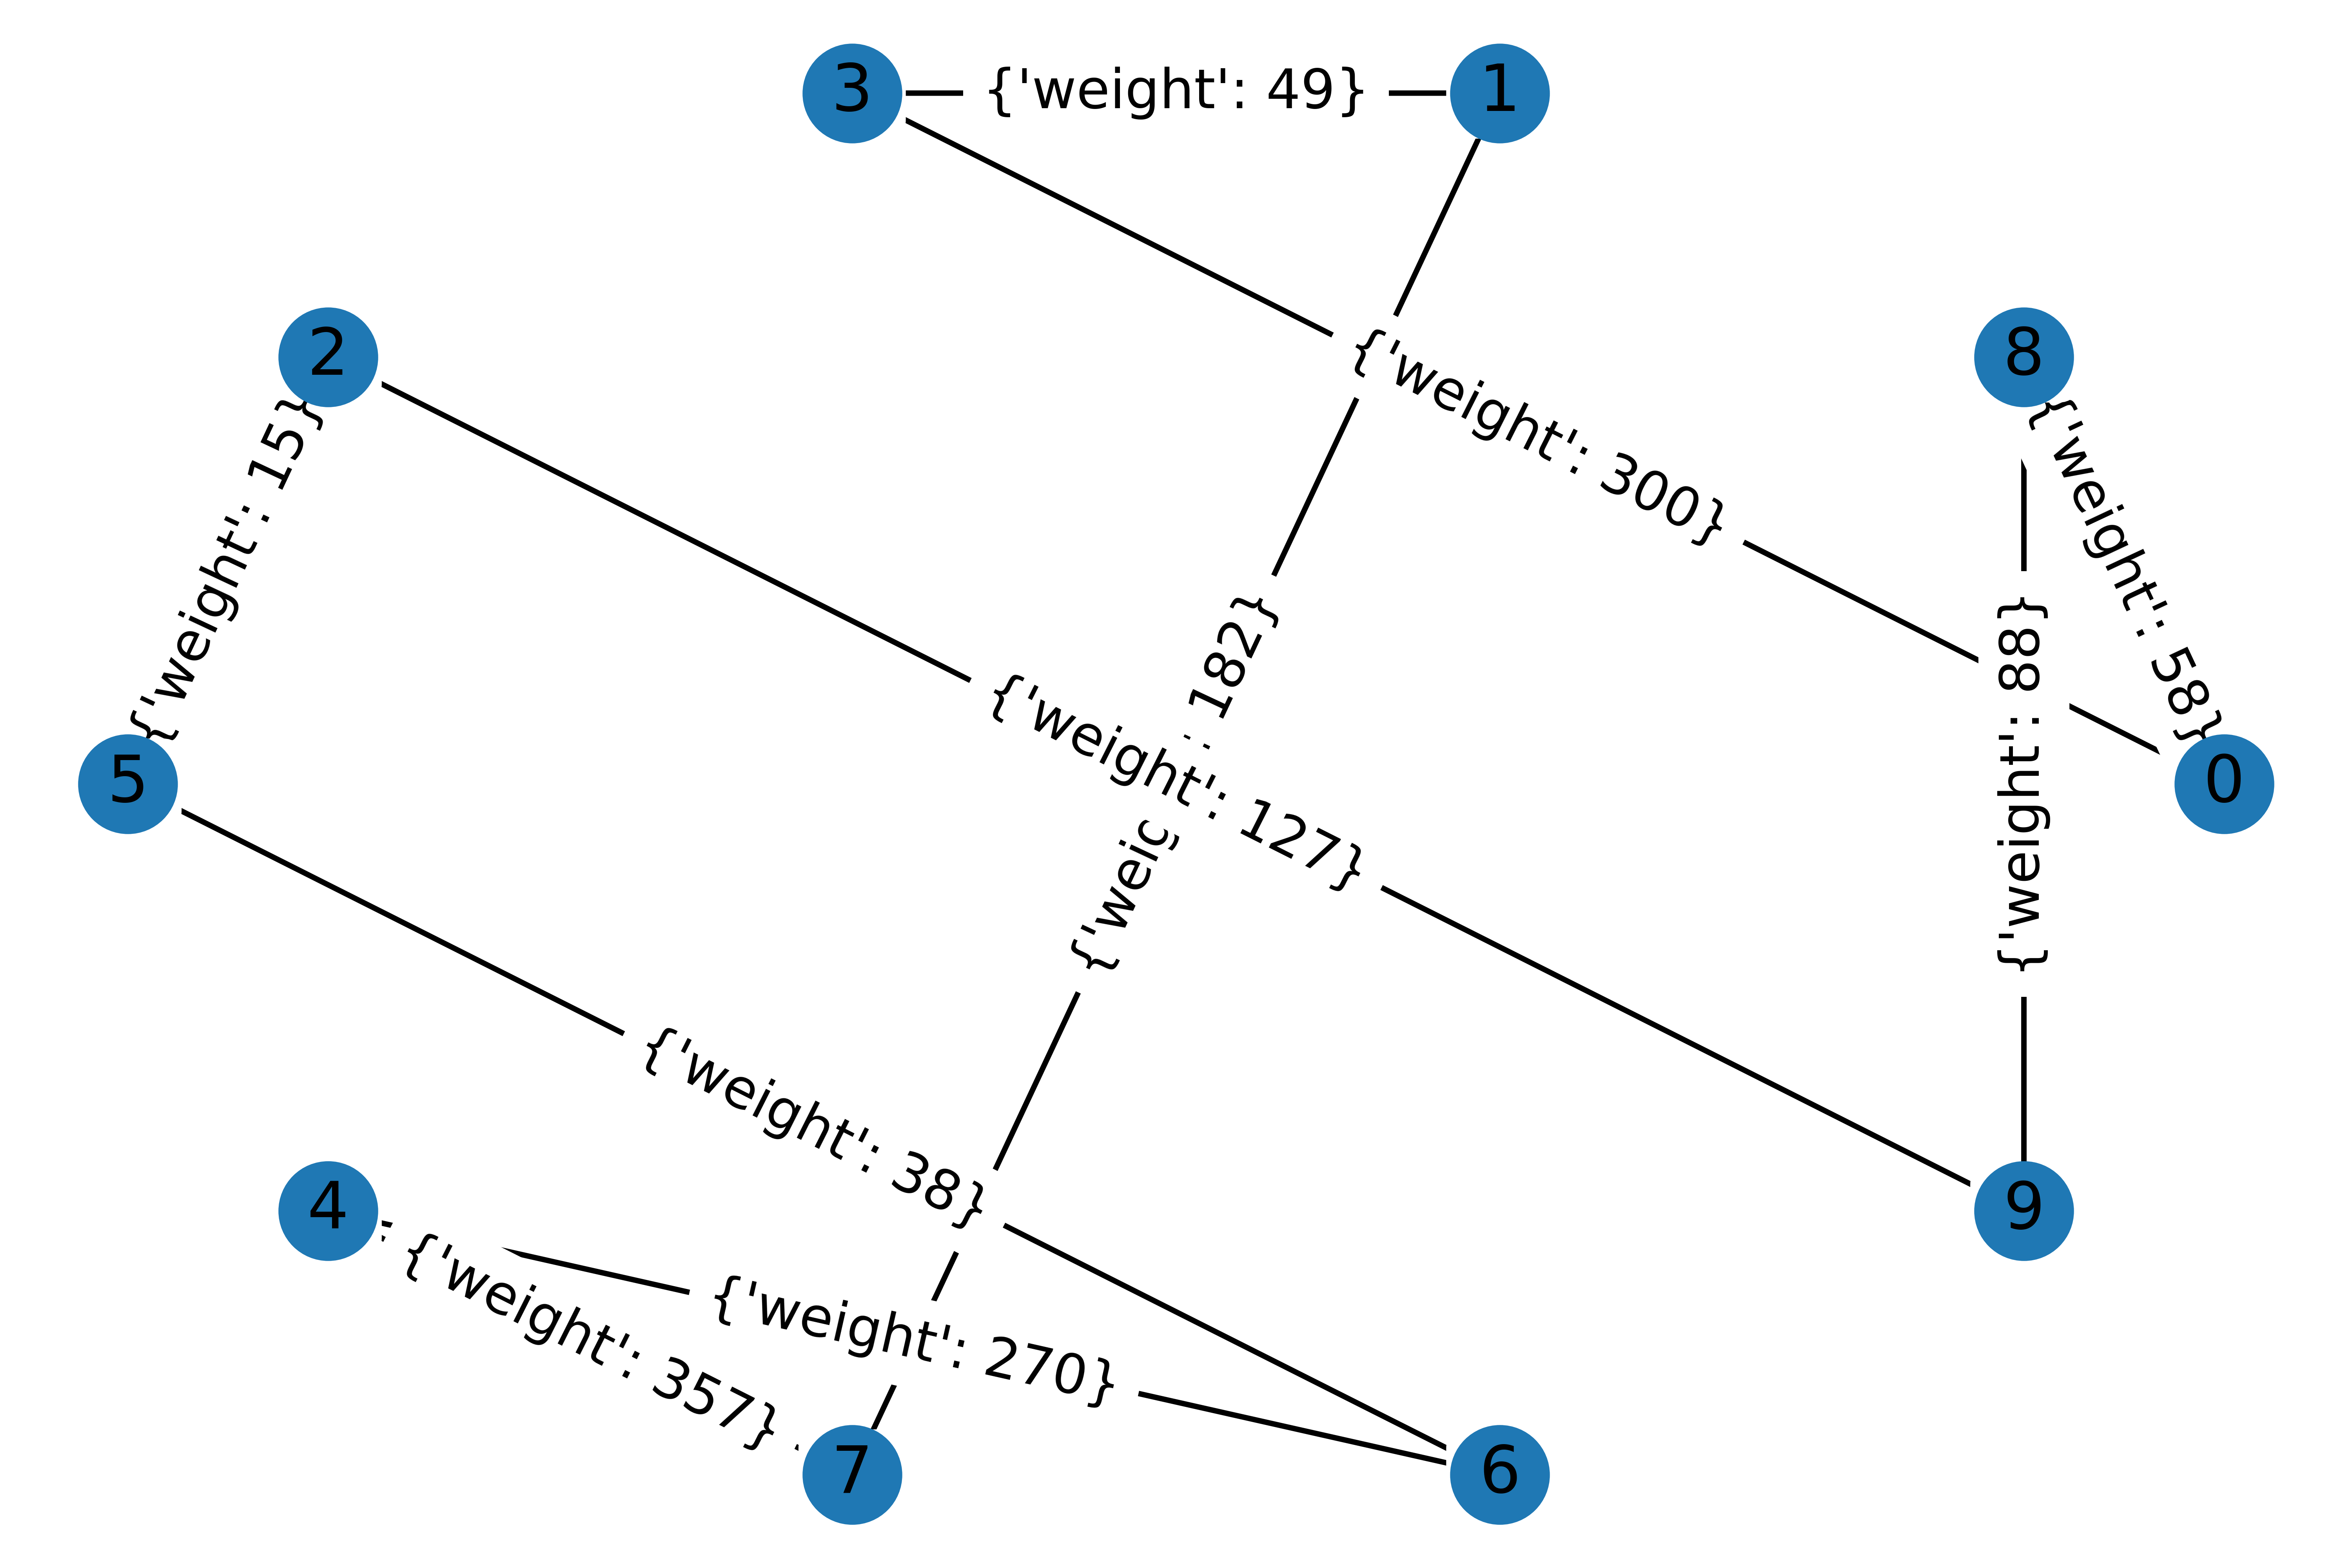
\includegraphics[width=0.8\linewidth]{primeri/primer2_lk.png}
\caption{LK}
\label{Slika 8}
\end{figure}
\end{minipage}
\end{columns}

\end{frame}


\end{document}